\subsection{Implementation Concepts}

\begin{figure}
\centering
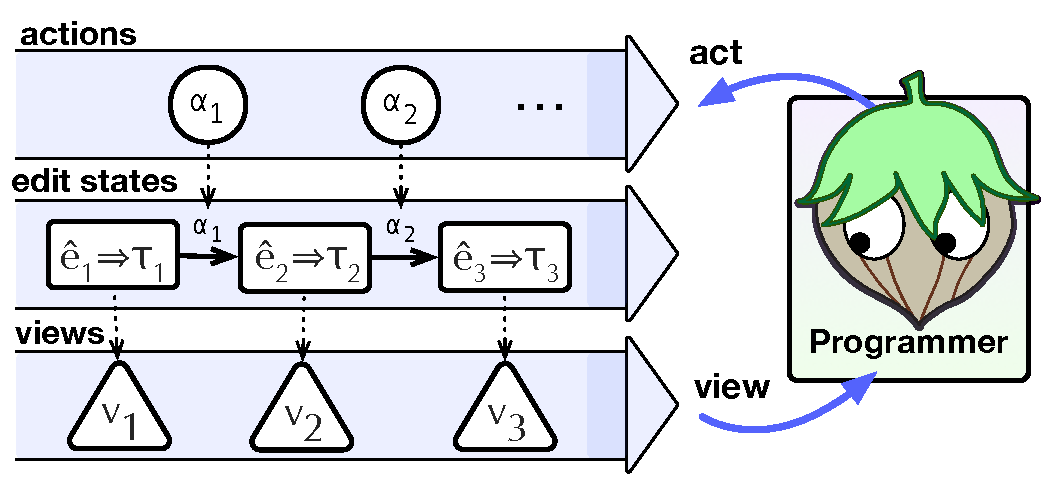
\includegraphics[width=0.90\columnwidth]{impl-overview2}
\caption{}
\label{fig:impl-overview}
\end{figure}











\todo{make figure take up only one column}\todo{change terminology in figure}\todo{revise}
The key question that must be answered for any implementation strategy is: how do we model a stream of actions from a user? Let us assume that these actions are chosen (using some input device, preferably, a keyboard) from some ``palette'' that never presents the user with actions that are not semantically well-defined, according to the action semantics defined earlier.
%In a traditional editor, the input from the user is a stream of characters, and there are no guarantees that at any point that the program is syntactically well-formed, so the designer leaves editing as an .
%In contrast, in a structure editor, the input from the user is a stream of operations.
As such, each new action will ``atomically'' generate a new Z-expression. 
This insight leads us to conclude that a natural way to implement this editor would be using event-based Functional Reactive Programming~\cite{Wan:2000:FRP:349299.349331} (FRP).
Figure~\ref{fig:FRP} illustrates the concept of an FRP-based implementation of a  structure editor organized like Hazelnut.
The input from the user is a stream of actions.  Each action results in a change to the underlying abstract model (i.e., a new Z-expression is created after each action.)
Each model change results in an updated \emph{view} which is then presented to the user.  The user can then consider this new view when they choose a new action as input.

\subsection{HZ}
We explore the concepts presented in the paper in HZ, our implementation of Hazelnut.
In order to reach a wide audience, we decided to implement HZ in the web browser.
In order to take advantage of all the benefits of FRP, we chose to implement HZ using OCaml\footnote{https://ocaml.org/}, the \texttt{js\_of\_ocaml} compiler\footnote{http://ocsigen.org/js\_of\_ocaml/} and the OCaml React library\footnote{http://erratique.ch/software/react}.

At the time of the writing of this paper, our implementation of HZ includes encodings of Z-expression as presented in this paper.
We consider this ZExp to be our model. 
HZ renders the model as a string embedded in HTML.
Currently we support only the delete action.  Other actions are currently under development. We anticipate having a substantially more functional implementation by the time this work is presented (our focus thusfar has been on the metatheory.) 
The work-in-progress code as well as directions for how to compile and run it can be found here: \url{https://github.com/hazelgrove/impl-tfp16}.

A substantially simpler system that we developed while exploring the ideas that led to Hazelnut can be found at the following URL:
\url{http://www.cs.cmu.edu/~comar/nestedpairs/}.
